\documentclass{beamer}
\usepackage{graphicx}
\usepackage{amssymb,amsfonts,amsmath}
% \usepackage{tikz,tkz-euclide}
\usepackage{subcaption}
% \usepackage{parskip}
% \usetikzlibrary{arrows.meta}
% \usetikzlibrary{calc,patterns}
\usefonttheme[onlymath]{serif}
% \usetheme{Berlin}
\title{Weekly Report}
\author{WU Zihan}
\begin{document}
\maketitle
\begin{frame}
    \frametitle{Outline}
    \tableofcontents
\end{frame}

\section{Experiment Results on Noisy Data}
\begin{frame}
    \frametitle{Results on Noisy Data}
    % two columns
    \begin{columns}
        \begin{column}{0.5\textwidth}
            \textbf{Settings}
            % smaller font
            \scriptsize
            \begin{itemize}
                \item $M = N = 10^4$
                \item $M_k = N_k \in \{50, 60, \dots, 190\}$
                \item $\kappa = \cfrac{\sigma^2}{B_{\max}} \in \{0.001 , 0.005, 0.01, 0.05, 0.1\}$
            \end{itemize}
            \textbf{Results}
            % figure result.png
            \begin{figure}[htb]
                \centering
                
\includegraphics[width=\linewidth]{result.png}
                \caption{Results on Noisy Data}
                \label{fig:results}
            \end{figure}
        \end{column}
        \begin{column}{0.5\textwidth}
            \vspace{-1cm}
            \centering
            \begin{figure}[htb]
                \centering
                \begin{subfigure}[b]{\textwidth}
                    \centering
                    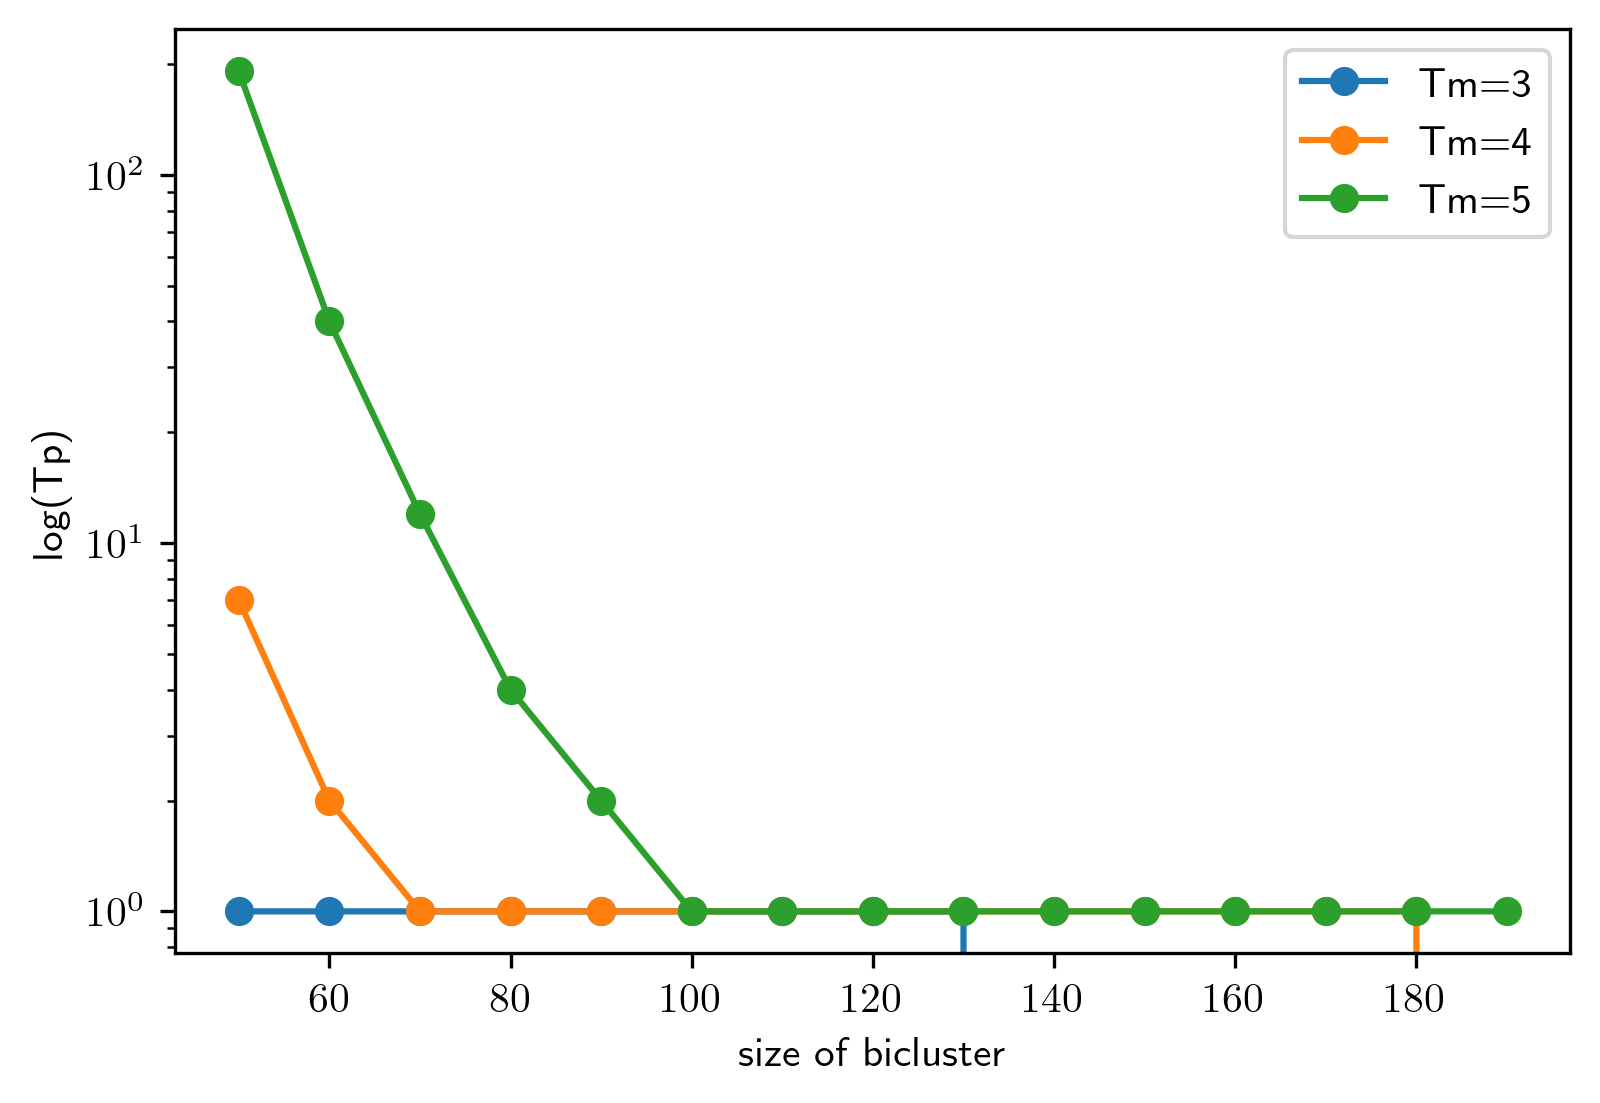
\includegraphics[width=\linewidth]{Tp.png}
                    \caption{Original matrix $A$}
                    \label{fig:image1}
                \end{subfigure}
                % \vspace{-0.5cm}
                \begin{subfigure}[b]{\textwidth}
                    \centering
                    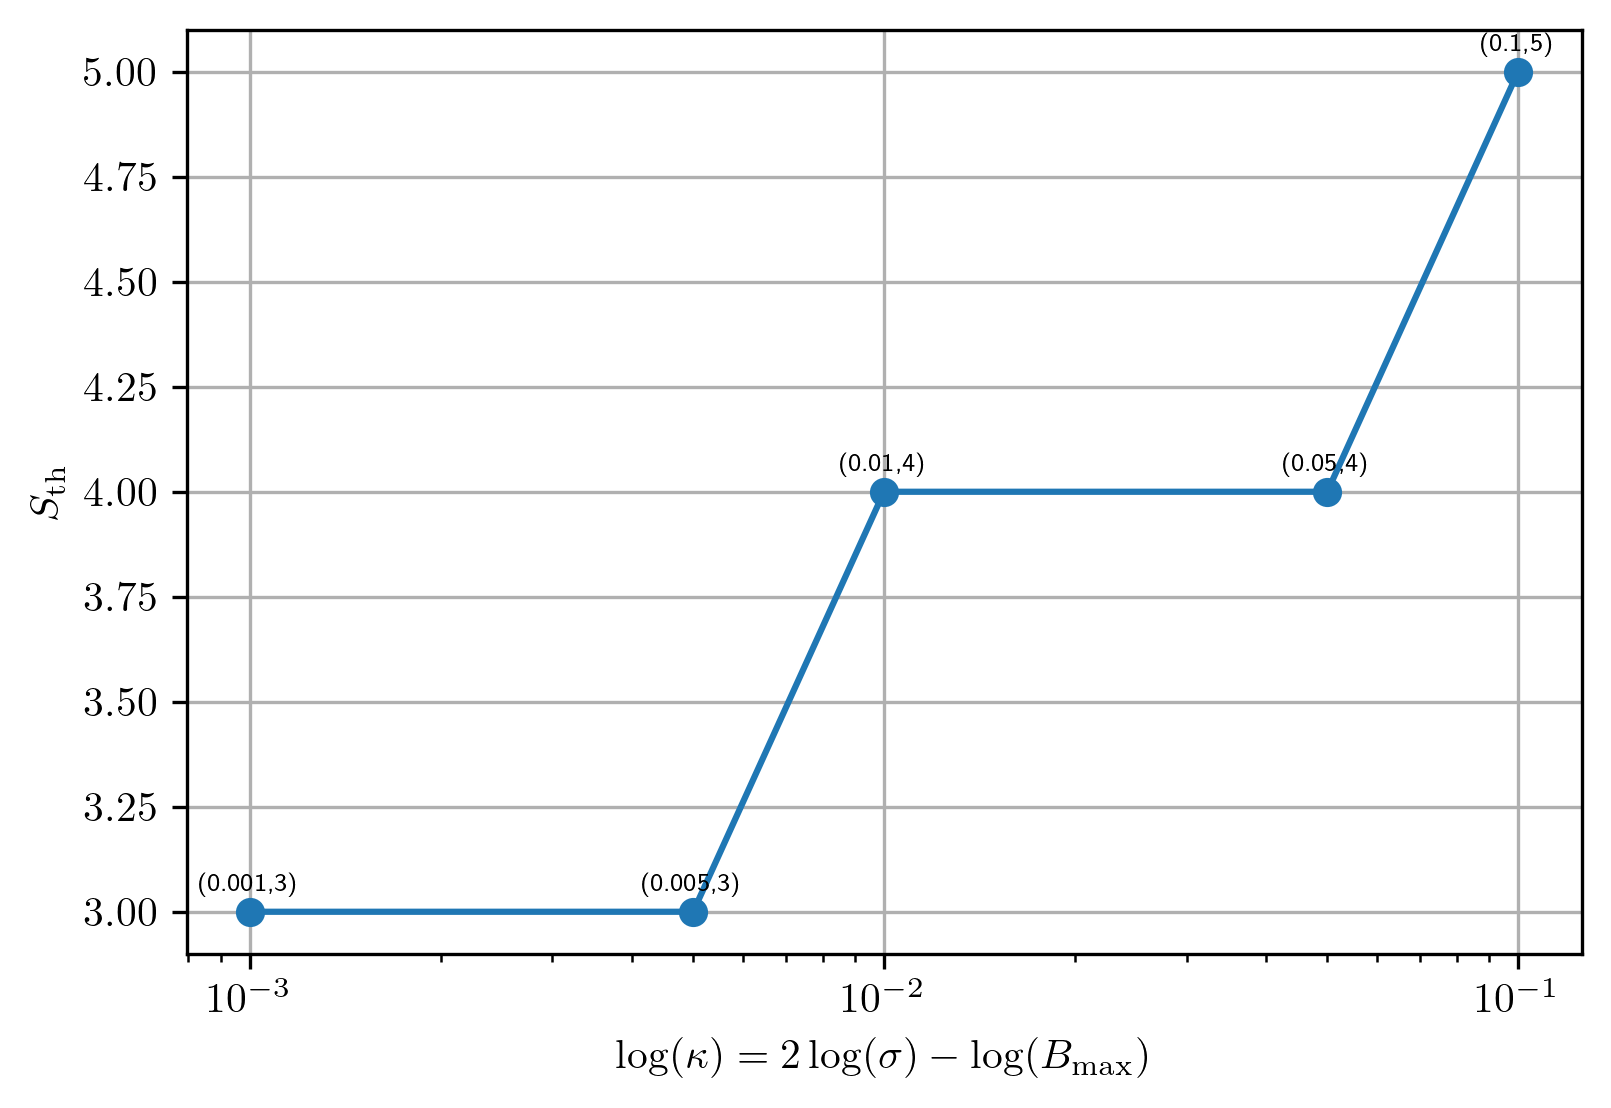
\includegraphics[width=\linewidth]{Tm.png}
                    \caption{Partition matrix $A$ into blocks}
                    \label{fig:image2}
                \end{subfigure}
                \vspace{-0.8cm}
                % \caption{Probability Model}
                % \label{fig:comparison}
            \end{figure}
        \end{column}
    \end{columns}

\end{frame}


\end{document}